\documentclass{article}
\usepackage[utf8]{inputenc}
\usepackage{amsmath}
\usepackage{amssymb}
\usepackage{graphicx}

\begin{document}
\section*{Hidden linear regression}
In this problem we consider the function $f\left(t\right) = \alpha e^{\beta t}$ with unknown parameters $\alpha > 0, \beta \in \mathbb{R}$. We are given measurement $\left(t_{i}, y_{i}\right)$ for $i = 1, \dots, n$ with $n > 2$. The goal is to determine $\alpha, \beta \in \mathbb{R}$ such that $f\left(t\right)$ fulfills the following condition as good as possible in the least square sense.
\begin{equation*}
    f\left(t_{i}\right) = y_{i}, \text{ with } y_{i} > 0, \: i = 1, \dots, n
\end{equation*}
\subsection*{3-1.a}
We are tasked with finding an overdetermined system of \textbf{nonlinear} equations from the above information. We have 
\begin{equation*}
    f\left(t_{i}\right) = y_{i} \Longleftrightarrow f\left(t_{i}\right) = \alpha e^{\beta t_{i}}
\end{equation*}
Hence the system of nonlinear equations is given by
\begin{align*}
   f\left(t_{1}\right) &= \alpha e^{\beta t_{1}} \\
   f\left(t_{2}\right) &= \alpha e^{\beta t_{2}} \\
   &\vdots \\
   f\left(t_{n}\right) &= \alpha e^{\beta t_{n}} 
\end{align*}
or in other notation
\begin{equation*}
    f\left(t_{i}\right) = \alpha e^{\beta t_{i}}, \: \: i = 1, \dots, n
\end{equation*}
where the non-linearity comes from $t_{i}$ appearing in the exponent of a term.
\subsection*{3-1.b}
We are now tasked with transforming this system of non-linear equations into an equivalent system of \textbf{linear} equations. Here we want $\alpha$ and $\beta$ to both appear as multiplicative or additive terms and not as exponents. Hence we apply the logarithm to both sides (which does not change the equality, as the logarithm is injective) to give us
\begin{align*}
 \log\left(f\left(t_{i}\right)\right) = \log\left(\alpha e^{\beta t_{i}}\right) &\Longleftrightarrow \log\left(f\left(t_{i}\right)\right) =\log\left(\alpha\right) + \log\left(e^{\beta t_{i}}\right) \\
 &\Longleftrightarrow \log\left(f\left(t_{i}\right)\right) =\log\left(\alpha\right) + \beta t_{i}
\end{align*}
Which hence gives us
\begin{equation*}
\log\left(f\left(t_{i}\right)\right) = \log\left(\alpha\right) + \beta t_{i}\,, \: \: i = 1, \dots, n
\end{equation*}
We hence define $g\left(t\right) := \log\left(f\left(t\right)\right)$ and $a := \log\left(\alpha\right)$. Which gives us the following overdetermined linear system of equations
\begin{equation}
    g\left(t_{i}\right) = a + \beta t_{i} \,, \: \: i = 1, \dots, n
\end{equation}

\pagebreak 

\subsection*{3-1.c}
We are tasked with writing down the normal equations for the overdetermined linear system of equations (1). We first construct the corresponding problem $\mathbf{A}\mathbf{x} = \mathbf{b}$.
\begin{equation*}
    \underbrace{\begin{bmatrix}
    1 & t_{1} \\
    1 & t_{2} \\
    \vdots \\
    1 & t_{n}
    \end{bmatrix}}_{=:\mathbf{A}}
    \underbrace{\begin{bmatrix}
        a \\ \beta
    \end{bmatrix}}_{=: \mathbf{x}}
    =
    \underbrace{\begin{bmatrix}
        g\left(t_{1}\right) \\
        g\left(t_{2}\right) \\
        \vdots \\
        g\left(t_{n}\right)
    \end{bmatrix}}_{=:\mathbf{b}}
\end{equation*}
where the normal equations are given by
\begin{equation*}
    \mathbf{A}^{\mathsf{T}}\mathbf{A}\mathbf{x} = \mathbf{A}^{\mathsf{T}}\mathbf{b}
\end{equation*}
Which we can express as
\begin{equation*}
\mathbf{A}^{\mathsf{T}}\mathbf{A}\mathbf{x} = 
\begin{bmatrix}
    1 & 1 & \dots & 1 \\
    t_{1} & t_{2} & \dots & t_{n}
\end{bmatrix}
    \begin{bmatrix}
    1 & t_{1} \\
    1 & t_{2} \\
    \vdots \\
    1 & t_{n}
    \end{bmatrix}
    = \begin{bmatrix}
        \sum_{i=1}^{n}1 & \sum_{i=1}^{n}t_{i} \\
        \sum_{i=1}^{n}t_{i} & \sum_{i=1}^{n}t_{i}^{2}
    \end{bmatrix} =
    \begin{bmatrix}
        n & \sum_{i=1}^{n}t_{i} \\
        \sum_{i=1}^{n}t_{i} & \sum_{i=1}^{n}t_{i}^{2}
    \end{bmatrix}
\end{equation*}
and (here we define $b_{i} = g\left(t_{1}\right)$)
\begin{equation*}
    \mathbf{A}^{\mathsf{T}}\mathbf{b} = \begin{bmatrix}
    1 & 1 & \dots & 1 \\
    t_{1} & t_{2} & \dots & t_{n}
\end{bmatrix} 
\begin{bmatrix}
    b_{1} \\
    b_{2} \\
        \vdots \\
    b_{n}
\end{bmatrix}
= 
\begin{bmatrix}
    \sum_{i=1}^{n}b_{i} \\
    \sum_{i=1}^{n}b_{i}t_{i}
\end{bmatrix}
\end{equation*}
\subsection*{3-1.d} 
We are now tasked with implementing a function \verb|linReg| that uses the method of normal equations to solve the general 1D linear regression problem for given inputs \verb|t| and \verb|y| which contain the corresponding points $\left(t_{i}, y_{i}\right)$. As per usual we use guidance from the lecture document in the form if the following code segement.
\begin{figure}[!hbt]
    \centering
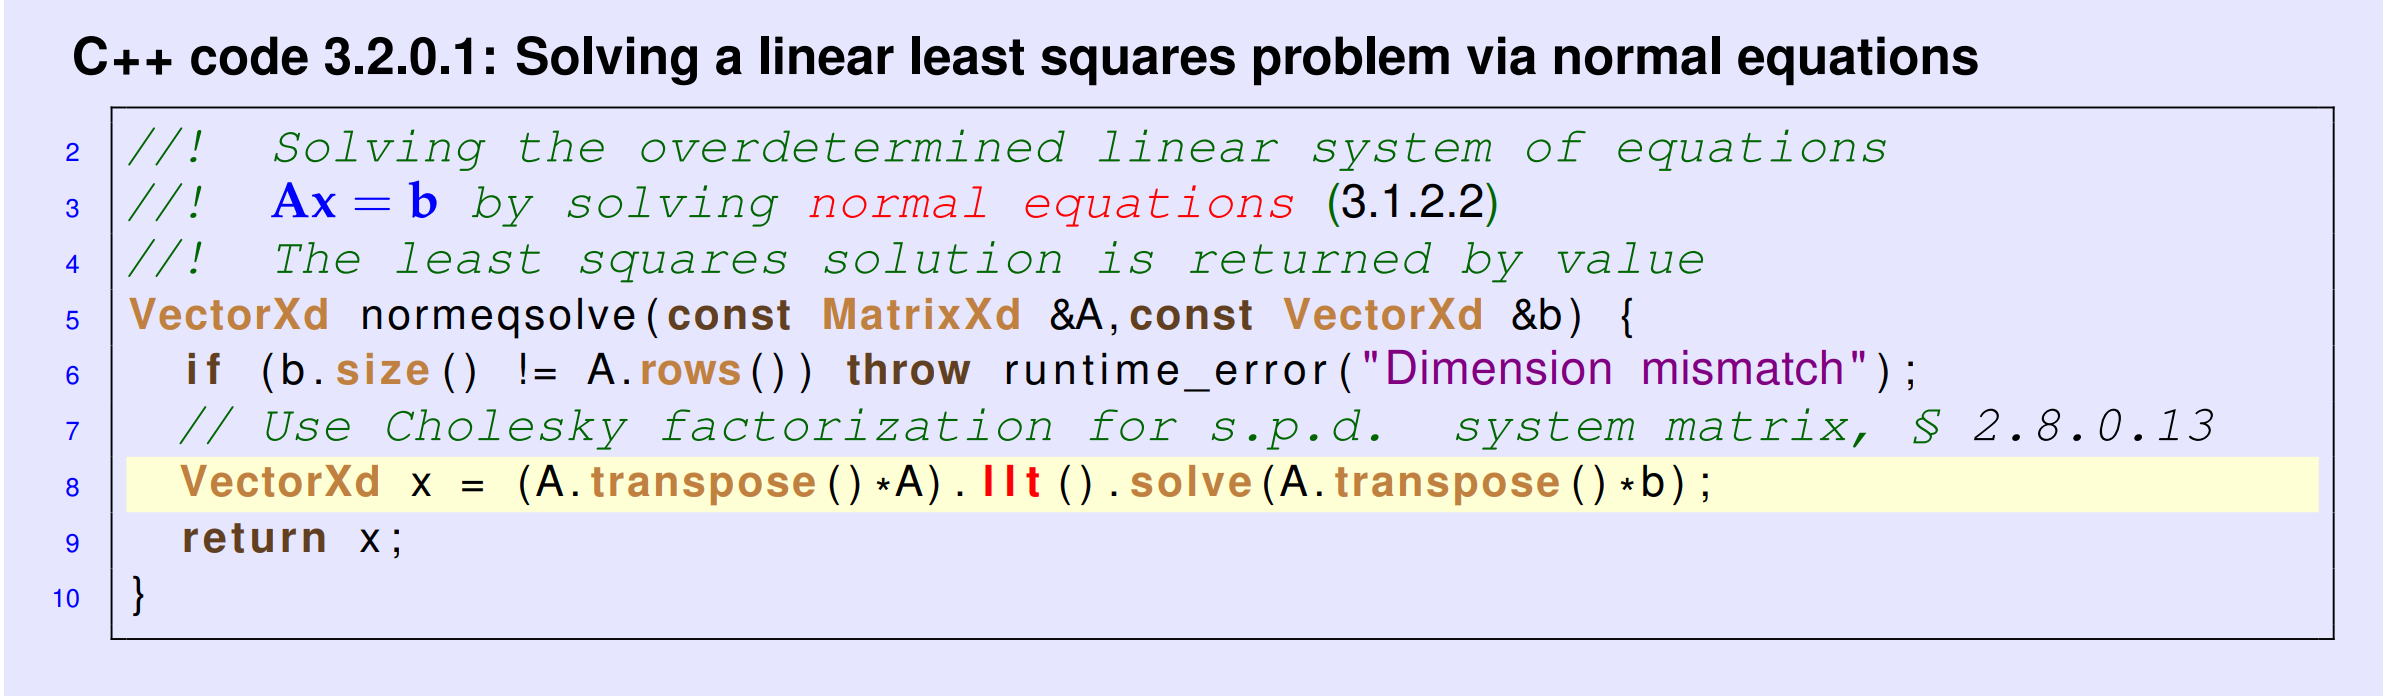
\includegraphics[width=1.0\linewidth]{NormalEquationsLinearLeastSquares.png}
\end{figure}

\pagebreak 

\noindent This gives us the following code.
\begin{figure}[!hbt]
    \centering
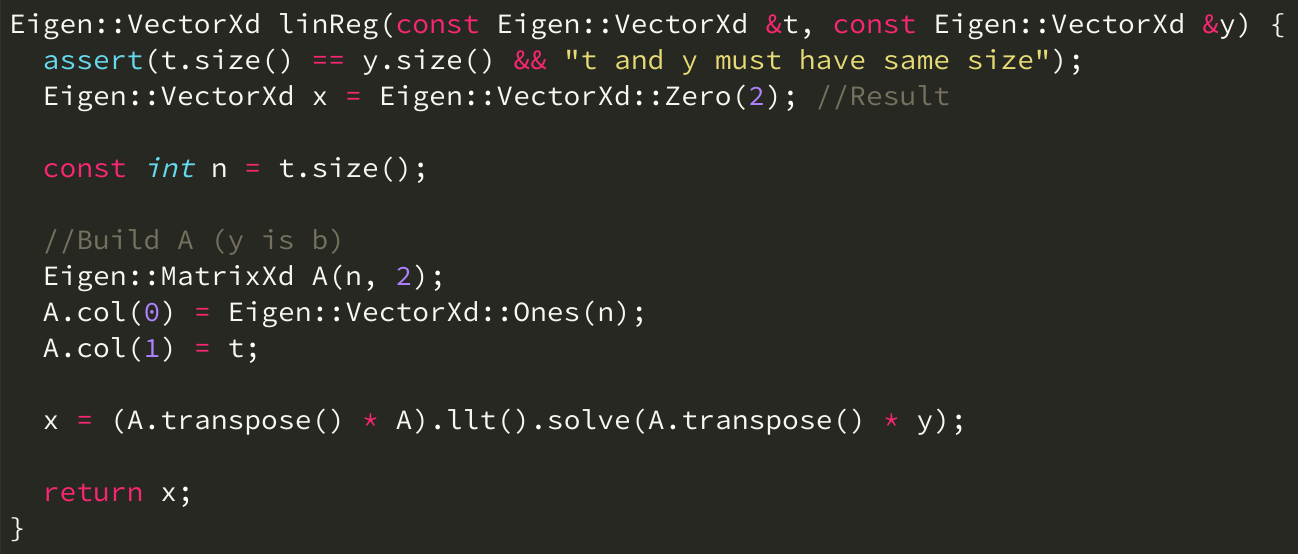
\includegraphics[width=1.0\linewidth]{3-1.d.png}
\end{figure}

\subsection*{3-1.e}
We are now tasked with solving the discussed nonlinear systems of equations using the discussed method of making it linear and the using the solver implemented in 3-1.d to do so. This results in the following code.
\begin{figure}[!hbt]
    \centering
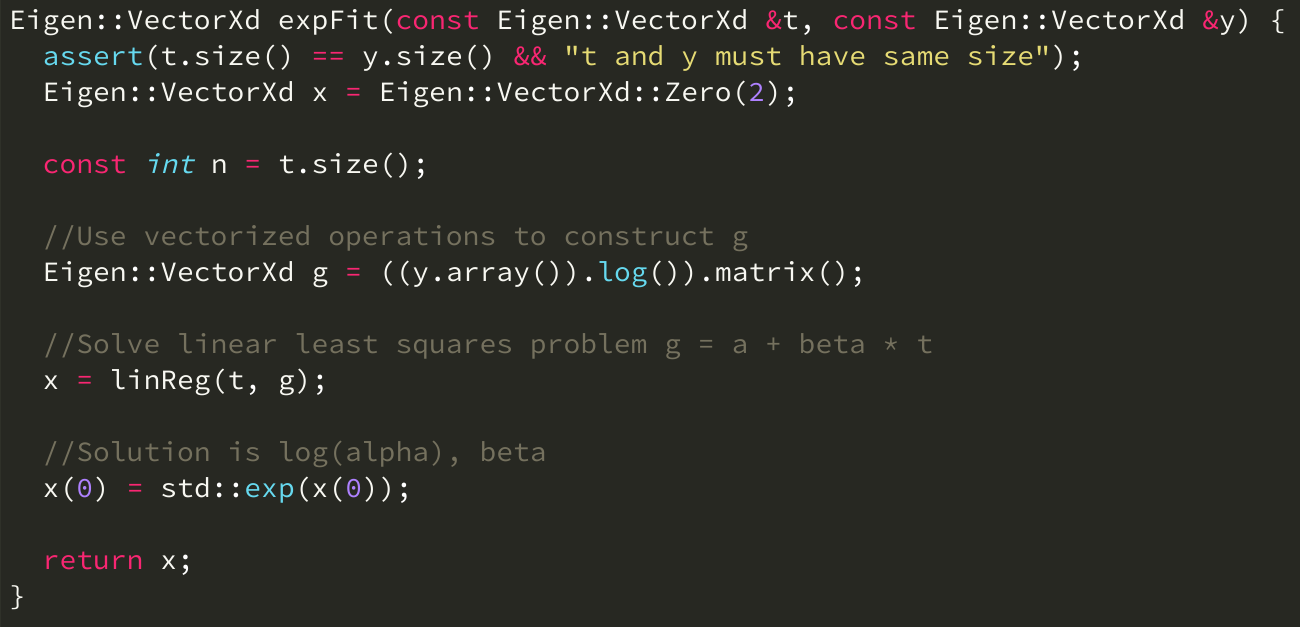
\includegraphics[width=1.0\linewidth]{3-1.e.png}
\end{figure}

\end{document}
